\chapter{Laws of Motion, Phase Space, and Conservation}

We begin, as Susskind does, with a wrong law. That is not antiquarian stage-setting. It is a way of asking what a law of motion is supposed to accomplish. A law should tell us how to move from one instant to the next, and a fundamental law ought also to preserve enough information that the past is not washed away by the future. Aristotle's law is close enough to ordinary friction-dominated experience to feel plausible, and precisely for that reason it is a good place to begin. By watching it fail, we see more sharply what Newton changes.

\section{Aristotle's Useful Wrong Law}

Aristotle lived in a world where friction is everywhere. Push an object and it moves; stop pushing and it stops. The heavier the object, the harder it is to give it a certain speed; the harder one pushes, the faster it goes. Out of that everyday experience comes the deliberately wrong law
\begin{equation}
\vec F=m\vec v.
\end{equation}
Susskind writes it down with some emphasis: this is the wrong equation. We are not to memorize it. We are to study it.

\begin{figure}
\centering

\includegraphics[width=0.82\textwidth]{lecture_02_figure_02.png}
\end{figure}

The point is not merely that Aristotle missed ice skating. The point is that he took force to be the source of motion itself, whereas Newton will make force the source of change of motion. But before correcting Aristotle, the lecture asks a more interesting question: in what sense is this even a law?

\section{From Force to an Update Rule}

To make that question precise, we pass at once to one dimension:
\begin{equation}
F=m\dot x.
\end{equation}
Now we enter what Susskind calls a stroboscopic world. Time is broken into small intervals of size \(\delta\), and the velocity is approximated by
\begin{equation}
\dot x(t)\approx \frac{x(t+\delta)-x(t)}{\delta}.
\end{equation}
Cleaning up the live board algebra, Aristotle's law becomes
\begin{align}
F(t)&=m\,\frac{x(t+\delta)-x(t)}{\delta},\\
x(t+\delta)&=x(t)+\frac{\delta}{m}F(t).
\end{align}
That is already a law of motion in a perfectly recognizable sense. If we know where the particle is at time \(t\), and if we know the force, then the law tells us where it will be at time \(t+\delta\).

This is the first important pivot of the lecture. A law becomes intelligible only when it becomes an update rule.

We can also read off the no-force case immediately. If \(F=0\), then \(\dot x=0\), so the object simply sits there:
\begin{equation}
F=0 \qquad \Rightarrow \qquad \dot x=0.
\end{equation}
In Aristotle's world, no force means no motion. The future is static, and so is the past.

\section{Aristotle's Spring and the Suspicion of Irreversibility}

Susskind now chooses the same example that later will be used again under Newton: a spring force. Suppose
\begin{equation}
F(x)=-kx.
\end{equation}
Insert this into Aristotle's update rule:
\begin{equation}
x(t+\delta)=x(t)-\frac{k\delta}{m}x(t)
=\left(1-\frac{k\delta}{m}\right)x(t).
\end{equation}
If \(\delta\) is small, then \(1-k\delta/m\) is slightly less than \(1\). So each time step multiplies the position by the same common factor. The motion is not oscillatory at all. The particle moves toward the origin, then closer, then closer still, shrinking by the same factor each step.

The continuous version says the same thing more cleanly. The sign in the spoken transcript wobbles a bit, but the intended equation is the one consistent with \(F=-kx\):
\begin{equation}
m\dot x=-kx.
\end{equation}
Its solution is
\begin{equation}
x(t)=x(0)e^{-kt/m}.
\end{equation}
So under Aristotle's law a displaced spring simply drifts back to equilibrium, slower and slower, exponentially decaying toward the origin. It does not swing through. It does not remember where it started except through an exponentially fading trace.

\subsection{Question \& Answer}

In what sense does Aristotle's law fail to predict the past?

Not in the trivial sense that the differential equation cannot be manipulated backward on paper. With infinite precision one can formally reconstruct earlier values. The lecture's point is subtler and more physical. Distinct initial conditions all flow into the same final resting state. If at a later time the particle is sitting essentially at the origin, then within any finite observational accuracy we can no longer tell where it came from. Initial distinctions are not preserved. Different histories collapse onto the same practical future.

This is why Susskind says Aristotle's law goes in the wrong direction from the point of view of reversibility. It predicts the future well enough, but it steadily loses information about the past.

\section{Newton's Law, Inertial Frames, and What the Law Really Says}

At this point the lecture turns. We now know what was really wrong with Aristotle. Force is not what makes an object move; force is what changes its state of motion. Friction itself is a force. In ordinary life the force from our hand often balances friction, and that balance can masquerade as a force-velocity law. But that is not a fundamental law.

Newton's second law is
\begin{equation}
F=m\ddot x.
\end{equation}
Before using it as a dynamical rule, Susskind pauses over inertial frames. The pause is brief but important. One should not be satisfied with the circular slogan that Newton's laws are true in inertial frames and inertial frames are the frames in which Newton's laws are true. The real statement is that there exist frames of reference in which Newton's laws hold. Those are the inertial frames. Other frames, accelerating or rotating relative to them, require extra structure.

He also pauses over the operational meaning of force and mass. A kilogram mass is identified by comparison with a standard mass. A spring balance gives meaning to a unit of force by a fixed amount of stretch. If one identical spring produces one unit of force, then two identical springs in parallel produce two units, and the acceleration doubles. If we keep the force fixed and double the mass, the acceleration is halved. In this way the statement
\begin{equation}
a\propto F,\qquad a\propto \frac{1}{m}
\end{equation}
is not empty symbolism. It is the content of experiment.

And now the lecture asks the same question it asked of Aristotle's law: is Newton's equation predictive?

\section{From Second Order to Phase Space}

If we discretize the second derivative in the standard way, we obtain
\begin{equation}
\ddot x(t)\approx \frac{x(t+\delta)-2x(t)+x(t-\delta)}{\delta^2}.
\end{equation}
The board algebra at this point is corrected in real time and is not worth following literally line by line. What matters is the cleaned update formula:
\begin{equation}
x(t+\delta)=2x(t)-x(t-\delta)+\frac{\delta^2}{m}F(t).
\end{equation}
Now a problem appears. To determine the next position, it is not enough to know the present position. We also need to know the earlier one. So Newton's law seems, at first glance, less predictive than Aristotle's.

\subsection{Question \& Answer}

If Newton's law is second order, why does it still count as a predictive law of motion?

Because the apparent defect lies not in Newton's law but in the way we have described the state. ``Knowing everything'' about a system cannot mean merely knowing its position. It must mean knowing whatever is needed to predict the future. Newton's law teaches us that the right initial data are position together with velocity. The second-order law is not a failure of predictiveness; it is a clue that the space of states is larger than configuration space alone.

That larger state space emerges when we introduce momentum:
\begin{equation}
p=m\dot x.
\end{equation}
Susskind writes this on the board and immediately rewrites Newton's law in terms of it.

\begin{figure}
\centering

\includegraphics[width=0.82\textwidth]{lecture_02_figure_03.png}
\end{figure}

Since the mass is taken to be constant in Newtonian mechanics, we have
\begin{equation}
\dot p = F,
\end{equation}
or in vector form,
\begin{equation}
\vec F=\frac{d\vec p}{dt}.
\end{equation}
The second law has become one first-order equation. The definition of momentum gives the other:
\begin{equation}
\dot x=\frac{p}{m}.
\end{equation}
So Newtonian mechanics in one dimension may be written as the pair
\begin{align}
\dot p&=F,\\
\dot x&=\frac{p}{m}.
\end{align}

\begin{figure}
\centering

\includegraphics[width=0.82\textwidth]{lecture_02_figure_04.png}
\end{figure}

In discrete language these become update rules,
\begin{align}
p(t+\delta)&=p(t)+\delta\,F(t),\\
x(t+\delta)&=x(t)+\frac{\delta}{m}p(t),
\end{align}
to first order in \(\delta\). One equation tells us how the momentum changes if we know the force. The other tells us how the position changes if we know the momentum. If the force is given as a function of position rather than explicitly as a function of time, nothing essential changes: once \(x\) and \(p\) are known at an instant, the force is known too, and the update goes through.

The state of the particle is therefore not just \(x\), but
\begin{equation}
(x,p),
\end{equation}
or equivalently \((x,\dot x)\). This enlarged space of initial data is phase space. The lecture stresses that point very strongly: phase space is the space of what one must know in order to predict the future.

\section{The Harmonic Oscillator and Time Reversal}

Now Susskind goes back to the spring and does the analogous Newtonian problem. This is not just another example. It is the same example under a different law, and therefore it reveals the structural difference between Aristotle and Newton with great clarity.

For the spring we have
\begin{equation}
m\ddot x=-kx.
\end{equation}
To keep the logic clear, let us set \(m=1\) and \(k=1\). Then
\begin{equation}
\ddot x=-x.
\end{equation}
The solutions are sines and cosines. A convenient form is
\begin{equation}
x(t)=c\cos(t-t_0),
\end{equation}
where \(c\) and \(t_0\) are the two constants of integration. Differentiating gives
\begin{equation}
\dot x(t)=-c\sin(t-t_0).
\end{equation}
Since \(m=1\), the momentum is equal to the velocity, so
\begin{equation}
p(t)=-c\sin(t-t_0).
\end{equation}
The sign of the trigonometric function is not the main point; the invariant relation is. Compute
\begin{equation}
x^2+p^2
=c^2\cos^2(t-t_0)+c^2\sin^2(t-t_0)
=c^2.
\end{equation}
Thus the motion in phase space lies on a circle:
\begin{equation}
x^2+p^2=c^2.
\end{equation}

That is the decisive contrast with Aristotle's spring. Under Aristotle's law all trajectories drift into the origin. Under Newton's law different initial conditions live on different cycles. Large displacements give large circles, small displacements give small circles, but no trajectory collapses onto any other. The past is not lost.

Project the motion onto the \(x\)-axis and we see the ordinary oscillation back and forth. Project it onto the \(p\)-axis and we see the momentum oscillate as well. When \(x\) is maximal, \(p=0\). When the particle passes through the origin, the momentum is maximal. Position and momentum are exchanged back and forth, but the orbit in phase space remains fixed. In this normalization all circles are traversed with the same period; only the radius and the starting point change.

The lecture then gives another view of reversibility. Under time reversal,
\begin{equation}
t\mapsto -t,\qquad \dot x\mapsto -\dot x,\qquad \ddot x\mapsto \ddot x.
\end{equation}
A first derivative changes sign, but a second derivative does not. So Aristotle's law is not invariant under reversal of time, whereas Newton's law is. If we film a Newtonian motion and run the film backward, we obtain another motion allowed by the same law.

A student asks why reversibility should be expected at all. Susskind's answer is deliberately modest. We are looking at successful laws of physics, searching for common structural features, and reversibility appears as one of them. At a deeper level the logical order runs the other way: Newtonian mechanics is an approximation emerging from more fundamental physics. But in this course we are proceeding from simple principles upward, and reversibility is one of the principles worth tracking.

\section{Conservation Laws: Momentum, Energy, and Potential}

The lecture now broadens from reversibility to conserved quantities. The harmonic oscillator has already suggested the idea: motion stays on one cycle and never jumps to another. That means there must be a label attached to the orbit. Susskind next derives two such labels, first momentum and then energy.

We begin with Newton's third law. Let \(\vec F_{ij}\) denote the force on particle \(i\) due to particle \(j\). Then
\begin{equation}
\vec F_{ij}=-\vec F_{ji}.
\end{equation}
Susskind also remarks that real interparticle forces are directed along the line joining the particles, but he explicitly postpones that part of the discussion to the later treatment of angular momentum. For momentum conservation, the crucial point is equal and opposite pairs.

For a closed system of particles,
\begin{equation}
\dot{\vec p}_i=\sum_{j\ne i}\vec F_{ij}.
\end{equation}
Now sum over all \(i\):
\begin{equation}
\frac{d}{dt}\sum_i \vec p_i=\sum_i\sum_{j\ne i}\vec F_{ij}.
\end{equation}
Each pair \(\vec F_{ij}\) and \(\vec F_{ji}\) appears once each and cancels. Therefore
\begin{equation}
\frac{d\vec P_{\text{tot}}}{dt}=0,
\end{equation}
where
\begin{equation}
\vec P_{\text{tot}}=\sum_i \vec p_i.
\end{equation}
So total momentum is conserved.

After that first conservation law, the lecture returns to a single particle and asks for energy conservation. We begin in one dimension, with a force that depends only on position:
\begin{equation}
F=F(x).
\end{equation}
Susskind is careful here. ``Time independent'' means not that the force cannot vary in time, but that its time dependence comes only through the particle's changing position. If the particle is at position \(x\), the force is \(F(x)\), no matter when that occurs.

In one dimension, for a sufficiently well-behaved force, we can always write
\begin{equation}
F(x)=-\frac{dV(x)}{dx},
\end{equation}
with
\begin{equation}
V(x)=-\int^x F(u)\,du+\text{const}.
\end{equation}
The minus sign is a convention, but it is a useful one: it makes the force point toward decreasing potential. The lecture asks us to picture a particle moving along the \(x\)-axis on a terrain of hills and valleys whose height is \(V(x)\). The steeper the hill, the larger the force; the force points downhill.

Now define the energy
\begin{equation}
E=\frac12 m\dot x^2+V(x).
\end{equation}
Here the first term is kinetic energy and the second is potential energy. Susskind emphasizes that, for present purposes, ``energy'' is simply the name we give to a conserved quantity if it turns out to be conserved.

\begin{figure}
\centering

\includegraphics[width=0.82\textwidth]{lecture_02_figure_05.png}
\end{figure}

Let us differentiate \(E\):
\begin{align}
\frac{dE}{dt}
&=\frac{d}{dt}\left(\frac12 m\dot x^2\right)+\frac{dV}{dt}\\
&=m\dot x\,\ddot x+\frac{dV}{dx}\dot x\\
&=\dot x\left(m\ddot x+\frac{dV}{dx}\right).
\end{align}
Now Newton's law says \(m\ddot x=F\), and the potential relation says \(F=-dV/dx\). Therefore
\begin{equation}
m\ddot x+\frac{dV}{dx}=0,
\end{equation}
so
\begin{equation}
\frac{dE}{dt}=0.
\end{equation}
That is energy conservation in one dimension. As the particle rolls downhill, \(V\) decreases while the kinetic term increases; as it climbs, the opposite occurs. The proof is simply the exact version of that intuitive trade-off.

For the spring force,
\begin{equation}
F=-kx,
\end{equation}
we obtain
\begin{equation}
\frac{dV}{dx}=kx,
\end{equation}
so
\begin{equation}
V(x)=\frac{k}{2}x^2.
\end{equation}
The total energy of the oscillator is therefore
\begin{equation}
E=\frac12 m\dot x^2+\frac{k}{2}x^2.
\end{equation}

\subsection{Question \& Answer}

Is every force field the gradient of a potential energy?

In one dimension, for nice enough \(F(x)\), essentially yes: any such function can be integrated, and so one can define a potential. But in several dimensions the situation changes completely. If we are given three independent force components \(F_1,F_2,F_3\), there is no mathematical necessity that they arise as partial derivatives of a single scalar \(V\). In one dimension the existence of \(V\) is nearly automatic; in several dimensions it is a genuine physical assumption.

That is exactly the obstacle Susskind wants to raise before resolving it by postulate.

\begin{figure}
\centering

\includegraphics[width=0.82\textwidth]{lecture_02_figure_06.png}
\end{figure}

For one particle in several coordinates \(\mathbf{x}=(x_1,\dots,x_n)\), Newton's law reads componentwise
\begin{equation}
F_i(\mathbf{x})=m\ddot x_i.
\end{equation}
What we would like to assume is
\begin{equation}
F_i(\mathbf{x})=-\frac{\partial V(\mathbf{x})}{\partial x_i},
\end{equation}
or, more compactly,
\begin{equation}
\vec F=-\nabla V.
\end{equation}
This says that the force points in the direction of steepest descent of the potential. The contour-map picture on the board is precisely the picture of a scalar potential together with the downhill direction.

\begin{figure}
\centering
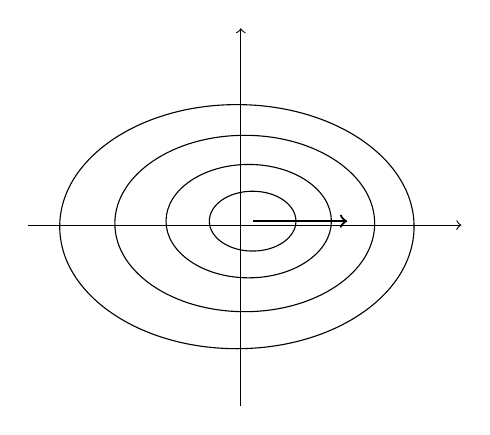
\begin{tikzpicture}[scale=1.0]
\draw[->] (-2.7,0) -- (2.8,0);
\draw[->] (0,-2.3) -- (0,2.5);
\draw (0.15,0.05) ellipse (0.55 and 0.38);
\draw (0.10,0.05) ellipse (1.05 and 0.72);
\draw (0.05,0.02) ellipse (1.65 and 1.12);
\draw (-0.05,-0.02) ellipse (2.25 and 1.55);
\draw[->,line width=0.8pt] (0.15,0.05) -- (1.35,0.05);
\end{tikzpicture}
\end{figure}

Once we assume this conservative-force form, the multidimensional energy is
\begin{equation}
E=\frac12 m\sum_i \dot x_i^2+V(x_1,\dots,x_n).
\end{equation}
Its time derivative is
\begin{align}
\frac{dE}{dt}
&=m\sum_i \dot x_i\ddot x_i+\frac{dV}{dt}\\
&=m\sum_i \dot x_i\ddot x_i+\sum_i\frac{\partial V}{\partial x_i}\dot x_i\\
&=\sum_i \dot x_i\left(m\ddot x_i+\frac{\partial V}{\partial x_i}\right).
\end{align}
If \(m\ddot x_i=F_i\) and \(F_i=-\partial V/\partial x_i\), then each bracket vanishes:
\begin{equation}
\frac{dE}{dt}=0.
\end{equation}
So energy is conserved in several dimensions as well, but now we must admit that we have paid a price. Unlike the one-dimensional case, we have made a real physical assumption: that the force components come from one scalar potential.

The many-particle generalization is then only a matter of bookkeeping. We flatten all coordinates of all particles into a single list \(x_1,\dots,x_{3N}\), allow corresponding masses \(m_i\), and define
\begin{equation}
E=\sum_{i=1}^{3N}\frac12 m_i\dot x_i^2+V(x_1,\dots,x_{3N}).
\end{equation}
If the force components satisfy
\begin{equation}
F_i=-\frac{\partial V}{\partial x_i},
\end{equation}
then exactly the same indexed derivation shows that the total energy of the whole system is conserved.

Susskind closes this part of the lecture by coming back one last time to the harmonic oscillator. For the spring,
\begin{equation}
V(x)=\frac{k}{2}x^2,
\end{equation}
so
\begin{equation}
E=\frac12 m\dot x^2+\frac{k}{2}x^2.
\end{equation}
When \(m=k=1\), this reduces to
\begin{equation}
E=\frac12\left(\dot x^2+x^2\right).
\end{equation}
But earlier we found
\begin{equation}
x^2+p^2=c^2,
\end{equation}
and in the normalization \(m=1\) we have \(p=\dot x\). Therefore the circles in phase space are nothing but contours of constant energy. The oscillator returns here not as a fresh example but as the payoff: the cycles in phase space are the level curves of the conserved quantity.

\section{Summary}

The lecture begins with Aristotle not to linger over a historical mistake, but to test what a law of motion should do. Aristotle's law becomes an update rule, predicts the future, and then reveals its weakness: distinct initial states collapse onto the same final rest state, so the past is not stably recoverable. Newton's law changes that by changing the very notion of state. Once we pass from position alone to phase space \((x,p)\), the second-order equation becomes a pair of first-order equations, and prediction is restored in the proper sense.

From there the spring becomes the central example twice over. Under Aristotle it decays. Under Newton it oscillates. In phase space it runs on circles, and those circles announce conserved quantities. Newton's third law yields conservation of total momentum. Conservative forces yield conservation of energy. In one dimension the potential description is almost automatic; in several dimensions it is a substantive law of nature. That is where the lecture leaves us: with phase space, with conservation laws, and with the harmonic oscillator already hinting at the more general formulations of mechanics still to come.